%% abtex2-modelo-artigo.tex, v-1.7.1 laurocesar
%% Copyright 2012-2013 by abnTeX2 group at http://abntex2.googlecode.com/ 
%%
%% This work may be distributed and/or modified under the
%% conditions of the LaTeX Project Public License, either version 1.3
%% of this license or (at your option) any later version.
%% The latest version of this license is in
%%   http://www.latex-project.org/lppl.txt
%% and version 1.3 or later is part of all distributions of LaTeX
%% version 2005/12/01 or later.
%%
%% This work has the LPPL maintenance status `maintained'.
%% 
%% The Current Maintainer of this work is the abnTeX2 team, led
%% by Lauro César Araujo. Further information are available on 
%% http://abntex2.googlecode.com/
%%
%% This work consists of the files abntex2-modelo-artigo.tex and
%% abntex2-modelo-references.bib
%%

% ------------------------------------------------------------------------
% ------------------------------------------------------------------------
% abnTeX2: Modelo de Artigo Acadêmico em conformidade com
% ABNT NBR 6022:2003: Informação e documentação - Artigo em publicação 
% periódica científica impressa - Apresentação
% ------------------------------------------------------------------------
% ------------------------------------------------------------------------

\documentclass[
	% -- opções da classe memoir --
	article,			% indica que é um artigo acadêmico
	12pt,				% tamanho da fonte
	twoside,			% para impressão apenas no verso. Oposto a twoside
	a4paper,			% tamanho do papel. 
	% -- opções da classe abntex2 --
	%chapter=TITLE,		% títulos de capítulos convertidos em letras maiúsculas
	%section=TITLE,		% títulos de seções convertidos em letras maiúsculas
	%subsection=TITLE,	% títulos de subseções convertidos em letras maiúsculas
	%subsubsection=TITLE % títulos de subsubseções convertidos em letras maiúsculas
	% -- opções do pacote babel --
	english,			% idioma adicional para hifenização
	brazil,				% o último idioma é o principal do documento
	]{abntex2}


% ---
% PACOTES
% ---

% ---
% Pacotes fundamentais 
% ---
\usepackage{cmap}				% Mapear caracteres especiais no PDF
\usepackage{lmodern}			% Usa a fonte Latin Modern
\usepackage[T1]{fontenc}		% Selecao de codigos de fonte.
\usepackage[utf8]{inputenc}		% Codificacao do documento (conversão automática dos acentos)
\usepackage{indentfirst}		% Indenta o primeiro parágrafo de cada seção.
\usepackage{nomencl} 			% Lista de simbolos
\usepackage{color}				% Controle das cores
\usepackage{graphicx}			% Inclusão de gráficos
\usepackage{amsmath}
% ---
\graphicspath{{imagens/}}
% ---
% Pacotes adicionais, usados apenas no âmbito do Modelo Canônico do abnteX2
% ---
\usepackage{lipsum}				% para geração de dummy text
% ---
		
% ---
% Pacotes de citações
% ---
\usepackage[brazilian,hyperpageref]{backref}	 % Paginas com as citações na bibl
\usepackage[alf]{abntex2cite}	% Citações padrão ABNT
% ---

% ---
% Configurações do pacote backref
% Usado sem a opção hyperpageref de backref
\renewcommand{\backrefpagesname}{Citado na(s) página(s):~}
% Texto padrão antes do número das páginas
\renewcommand{\backref}{}
% Define os textos da citação
\renewcommand*{\backrefalt}[4]{
	\ifcase #1 %
		Nenhuma citação no texto.%
	\or
		Citado na página #2.%
	\else
		Citado #1 vezes nas páginas #2.%
	\fi}%
% ---

% ---
% Informações de dados para CAPA e FOLHA DE ROSTO
% ---
\titulo{Trabalho Prático 2 \\ Geração de Números Aleatórios}
\autor{Grupo 13 \\ Alisson Moreira Ferreira - 11/0106946 \\ Augusto Cesar Ribeiro Nunes - 13/0103004}
\local{Brasil}
\data{16 de abril de 2016}
% ---

% ---
% Configurações de aparência do PDF final

% alterando o aspecto da cor azul
\definecolor{blue}{RGB}{41,5,195}

% informações do PDF
\makeatletter
\hypersetup{
     	%pagebackref=true,
		pdftitle={\@title}, 
		pdfauthor={\@author},
    	pdfsubject={Trabalho Prático 2 da Disciplina Estatística Computacional 2},
	    pdfcreator={LaTeX with abnTeX2},
		pdfkeywords={abnt}{latex}{abntex}{abntex2}{atigo científico}, 
		colorlinks=true,       		% false: boxed links; true: colored links
    	linkcolor=blue,          	% color of internal links
    	citecolor=blue,        		% color of links to bibliography
    	filecolor=magenta,      		% color of file links
		urlcolor=blue,
		bookmarksdepth=4
}
\makeatother
% --- 

% ---
% compila o indice
% ---
\makeindex
% ---

% ---
% Altera as margens padrões
% ---
\setlrmarginsandblock{4cm}{4cm}{*}
\setulmarginsandblock{4cm}{4cm}{*}
\checkandfixthelayout
% ---

% --- 
% Espaçamentos entre linhas e parágrafos 
% --- 

% O tamanho do parágrafo é dado por:
\setlength{\parindent}{1.3cm}

% Controle do espaçamento entre um parágrafo e outro:
\setlength{\parskip}{0.2cm}  % tente também \onelineskip

% Espaçamento simples
\SingleSpacing

% ----
% Início do documento
% ----
\begin{document}

% Retira espaço extra obsoleto entre as frases.
\frenchspacing 

% ----------------------------------------------------------
% ELEMENTOS PRÉ-TEXTUAIS
% ----------------------------------------------------------

%---
%
% Se desejar escrever o artigo em duas colunas, descomente a linha abaixo
% e a linha com o texto ``FIM DE ARTIGO EM DUAS COLUNAS''.
% \twocolumn[    		% INICIO DE ARTIGO EM DUAS COLUNAS
%
%---
% página de titulo
\maketitle

% resumo em português
\begin{resumoumacoluna}
    Este Trabalho Prático implementa um gerador variáveis aleatórias Uniformes no intervalo (0,1) utilizando o Método Congruencial em (\ref{metodo:runif_cong}), implementa a geração de variáveis aleatórias Normais padrão utilizando o Método polar em (\ref{metodo:rnorm_polar}), e constrói uma tabela para as probabilidades acumuladas da N(0,1) utilizando duas implementações: o Método de Integração de Monte-Carlo em (\ref{eq:pnorm_MC}) e a Probabilidade Acumulada Empírica obtida em (\ref{eq:rnorm_polar}) no item (\ref{eq:pnorm_polar})
 
 \vspace{\onelineskip}
 
 \noindent
\end{resumoumacoluna}

% ]  				% FIM DE ARTIGO EM DUAS COLUNAS
% ---

% ----------------------------------------------------------
% ELEMENTOS TEXTUAIS
% ----------------------------------------------------------
\textual

% ----------------------------------------------------------
% Introdução
% ----------------------------------------------------------
\section{Introdução}
    Técnicas de Simulação são amplamente utilizadas em Ciências Naturais, Biológicas e na Tecnologia. Os seus custos diminuíram drasticamente nas últimas décadas, e acompanharam a evolução da computação em sentido inverso: hoje podemos simular processos com alto grau de sensibilidade e especificidade até mesmo em nossos computadores pessoais, e não mais em \textit{mainframes} cujo acesso era restrito e o custo elevadíssimo.
    
    Nas Ciências Físicas, podemos citar os sofisticados Modelos Climáticos \cite{ramirez2007desempenho} que utilizam simulação para a obtenção de previsões com maior ou menor grau de sucesso\footnote{O próprio \textit{paper} em questão faz uma espécie de meta-análise de modelos do IPCC, GFDL e HAD}. Na Estatística, a aplicação mais conhecida de Técnicas de Simulação são as ligadas direta ou indiretamente aos chamados \textbf{Métodos de Monte-Carlo}. 
    
    Na Estatística, encontramos aplicações (sofisticadas) de Simulação em Técnicas de Redução de Variância (como Amostragem de Importância e Amostragem Antitética) e em Processos Estocásticos (Algoritmo de Metropolis-Hastings, Amostragem de Gibbs, e MCMC). Em um nível mais simples, qualquer programa de computação científica que se preze contém uma implementação de geradores de variáveis aleatórias, um uso mais simples de Simulação.
    
    
\section{Metodologia}

    Este Trabalho Prático aborda em um de seus tópicos a Integração Numérica utilizando Monte-Carlo. A ideia é a seguinte: sendo $g(x)$ uma função arbitrária, e supondo que desejamos obter uma aproximação numérica para $\theta$ onde 
    
    \begin{equation}\label{eq:mc_01}
      \theta = \int_0^1g(x)dx  
    \end{equation}
    
    
    podemos olhar para $\theta$ como a Esperança de uma função $g(U)$ com $U \sim U(0,1)$. Supondo $U_1,\dots,U_n$ variáveis aleatórias independentes e identicamente distribuídas com $U_i \sim U(0,1)$ para $i = 1,\dots,n$, segue que $g(U_1),\dots,g(U_n)$ são variáveis aleatórias independentes e identicamente distribuídas com média $\theta$. Portanto, pela Lei Forte dos Grandes Números, temos com Probabilidade 1 que 
    
    \begin{equation}\label{eq:LFGN_MC}
        \lim_{n \rightarrow \infty}\sum_{i=1}^n\frac{g(U_i)}{n} \rightarrow E[g(U)] = \theta, 
    \end{equation}
    
    Logo, nós podemos aproximar $\theta$ utilizando uma amostra \textit{grande} de $u_i$ tirados de uma distribuição Uniforme em $(0,1)$. Para o caso mais geral onde os limites inferior e superior da integral (\ref{eq:mc_01}) são $a$ e $b$ quaisquer ($a<b$), podemos aplicar a substituição $y = (x-a)/(b-a), dy = dx/(b-a)$, obtendo 
    \begin{equation}\label{eq:MCI_arb}
        \theta = \int_0^1g(a+[b-a]y)(b-a)dy = \int_0^1h(y)dy
    \end{equation}
    
    onde $h(y) = (b-a)g(a+[b-a]y)$. Portanto, podemos aproximar $\theta$ tomando uma amostra de variáveis aleatórias Uniformes em $(0,1)$ e tomando a média de $h$ avaliada nas observações da amostra. A última parte do trabalho consiste na criação de uma tabela para a densidade acumulada da Normal(0,1), i.e., vamos aproximar a integral $\int_0^b \frac{1}{2\pi}exp\{-\frac{x_i}{2\sigma^2}\}$ utilizando o Método de Monte Carlo para integração numérica. O método foi implementado pela função \textbf{pnorm\_MC()}, e os valores obtidos com este método são comparados com os obtidos pela função \textbf{pnorm()} do R.
    
    Inicialmente há a necessidade de implementação de um gerador de variáveis aleatórias para a distribuição Uniforme em $(0,1)$. Utilizou-se o \textbf{Método Congruencial Multiplicativo} para tal finalidade. O método em questão consiste em, a partir de uma semente \textit{aleatória}\footnote{Na verdade, a maior parte os geradores aleatórios implementados e utilizados habitualmente são pseudo-aleatórios. Ver \cite{wiki:001} [em inglês] para uma explicação mais detalhada.}, obter uma sequência de números aleatórios ${x_1,x_2,\dots}$ tomando $x_n = (ax_{n-1}) \mod m$, com $a$ e $m$ inteiros positivos. Este gerador foi implementado pela função \textbf{runif\_congruencial()}. 
    
    Um outro método para geração de variáveis aleatórias estudado neste Trabalho Prático é o Método Polar\footnote{Em particular, utilizamos aqui o que se chama de Método Polar de Marsaglia: ver }: este método gera pares de variáveis aleatórias contínuas utilizando uma transformação em coordenadas polares. Em particular, implementamos um gerador de variáveis aleatórias Normais padrão, e sua função é \textbf{rnorm\_polar()}. Em um segundo momento, a distribuição acumulada empírica utilizando este método também foi utilizada para gerar uma tabela dos quantis da Normal padrão, comparando-a com os resultados da função \textbf{pnorm()} do R.
    
    As implementações, os resultados dos testes de hipóteses e sementes utilizados para verificar o ajustamento dos geradores encontram-se no Anexo A. As funções foram documentadas utilizando o pacote \textit{Roxygen} do R. Disponibilizamos um repositório no site github.com: (http://github.com/august-o/TP2-EstComp). Lá encontram-se todos os arquivos-fonte utilizados neste Trabalho Prático. O computador utilizado foi um Macbook Pro, Sistema Operacional OS X El Capitan (10.11.3), com processador Intel Core i5 de 2.4 GHz e 16 GB de memória RAM 1333 MHz DDR3. A versão do R utilizada foi a 3.2.4, com a IDE RStudio em sua versão 0.99.786.  
    
\section{Gerador Congruencial para a variável aleatória Uniforme(0,1)}\label{metodo:runif_cong}
\subsection{Teste de Uniformidade}
    Com a implementação adotada e a amostra obtida (ver Anexo A), foram realizados três Testes de Hipóteses para 
        
    \begin{align*}
        H_0 & : X \sim U(0,1) \\
        H_1 & : X \sim T
    \end{align*}
    
    onde X é o vetor aleatório  ($n = 10^5$) gerado pela implementação utilizada, e T é uma distribuição qualquer que não seja a Uniforme(0,1). O \textbf{Teste de Kolmogorov-Smirnov} para a Uniformidade da Distribuição gerada não rejeita a hipótese nula a um nível de significância de 0.7253, o \textbf{Teste de Cramér-von Mises} não rejeita a hipótese nula a um nível de significância 0.7823, e o \textbf{Teste de Anderson-Darling} não rejeita a hipótese nula a um nível de significância de 0.5601. 
    
    Como verificação qualitativa, adicional, abaixo estão os histogramas do vetor usando o gerador congruencial e do vetor utilizando \textbf{runif()} do R. Note que ambos são \textit{uniformes} e muito similares\footnote{Isso é o máximo que se pode dizer numa inspeção visual para "verificar" esse tipo de similaridade.}

    \begin{figure}[h]
        \centering
        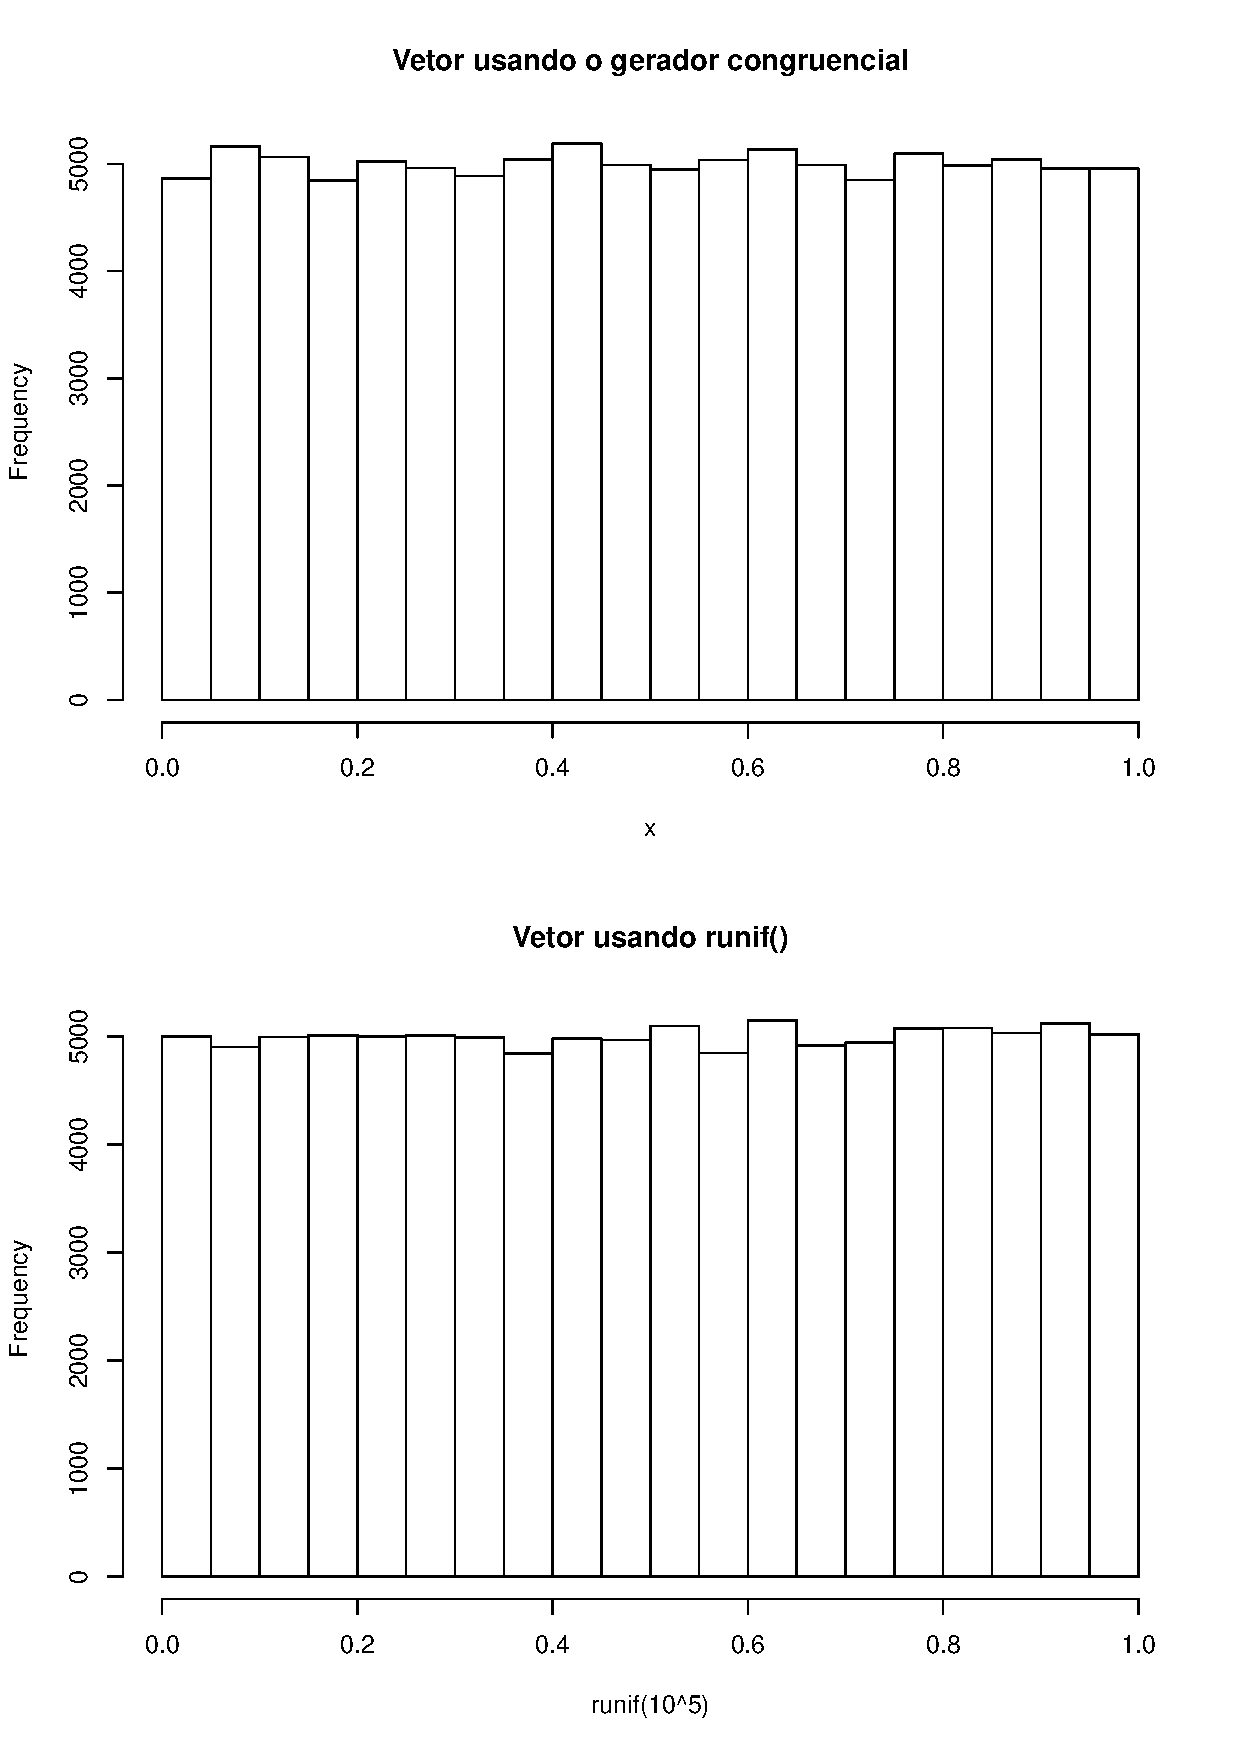
\includegraphics[scale=0.24]{hist_runif_congruencial}
        \caption{Histogramas para o gerador e para a função runif(), n = 10^5}
        \label{fig:hist_runif}
    \end{figure}
    
\section{Gerador Polar para a variável aleatória Normal Padrão}
\subsection{Teste de Normalidade}\label{metodo:rnorm_polar}
    Com a implementação adotada e a amostra obtida (ver Anexo A), foram realizados três Testes de Hipóteses para 
        
    \begin{align*}
        H_0 & : X \sim N(0,1) \\
        H_1 & : X \sim T
    \end{align*}
    
    onde X é o vetor aleatório  ($n = 10^7$) gerado pela implementação utilizada, e T é uma distribuição qualquer que não seja a Normal(0,1). O \textbf{Teste de Kolmogorov-Smirnov} para a Uniformidade da Distribuição gerada não rejeita a hipótese nula a um nível de significância de 0.8173, o \textbf{Teste de Cramér-von Mises} não rejeita a hipótese nula a um nível de significância 0.8573, e o \textbf{Teste de Anderson-Darling} não rejeita a hipótese nula a um nível de significância de 0.8223. 
    
    Como verificação qualitativa, adicional, abaixo estão os gráficos de densidade \textit{Kernel} do vetor usando o Método Polar de Marsaglia e do vetor utilizando \textbf{rnorm()} do R. 
    
    \begin{figure}[h]
        \centering
        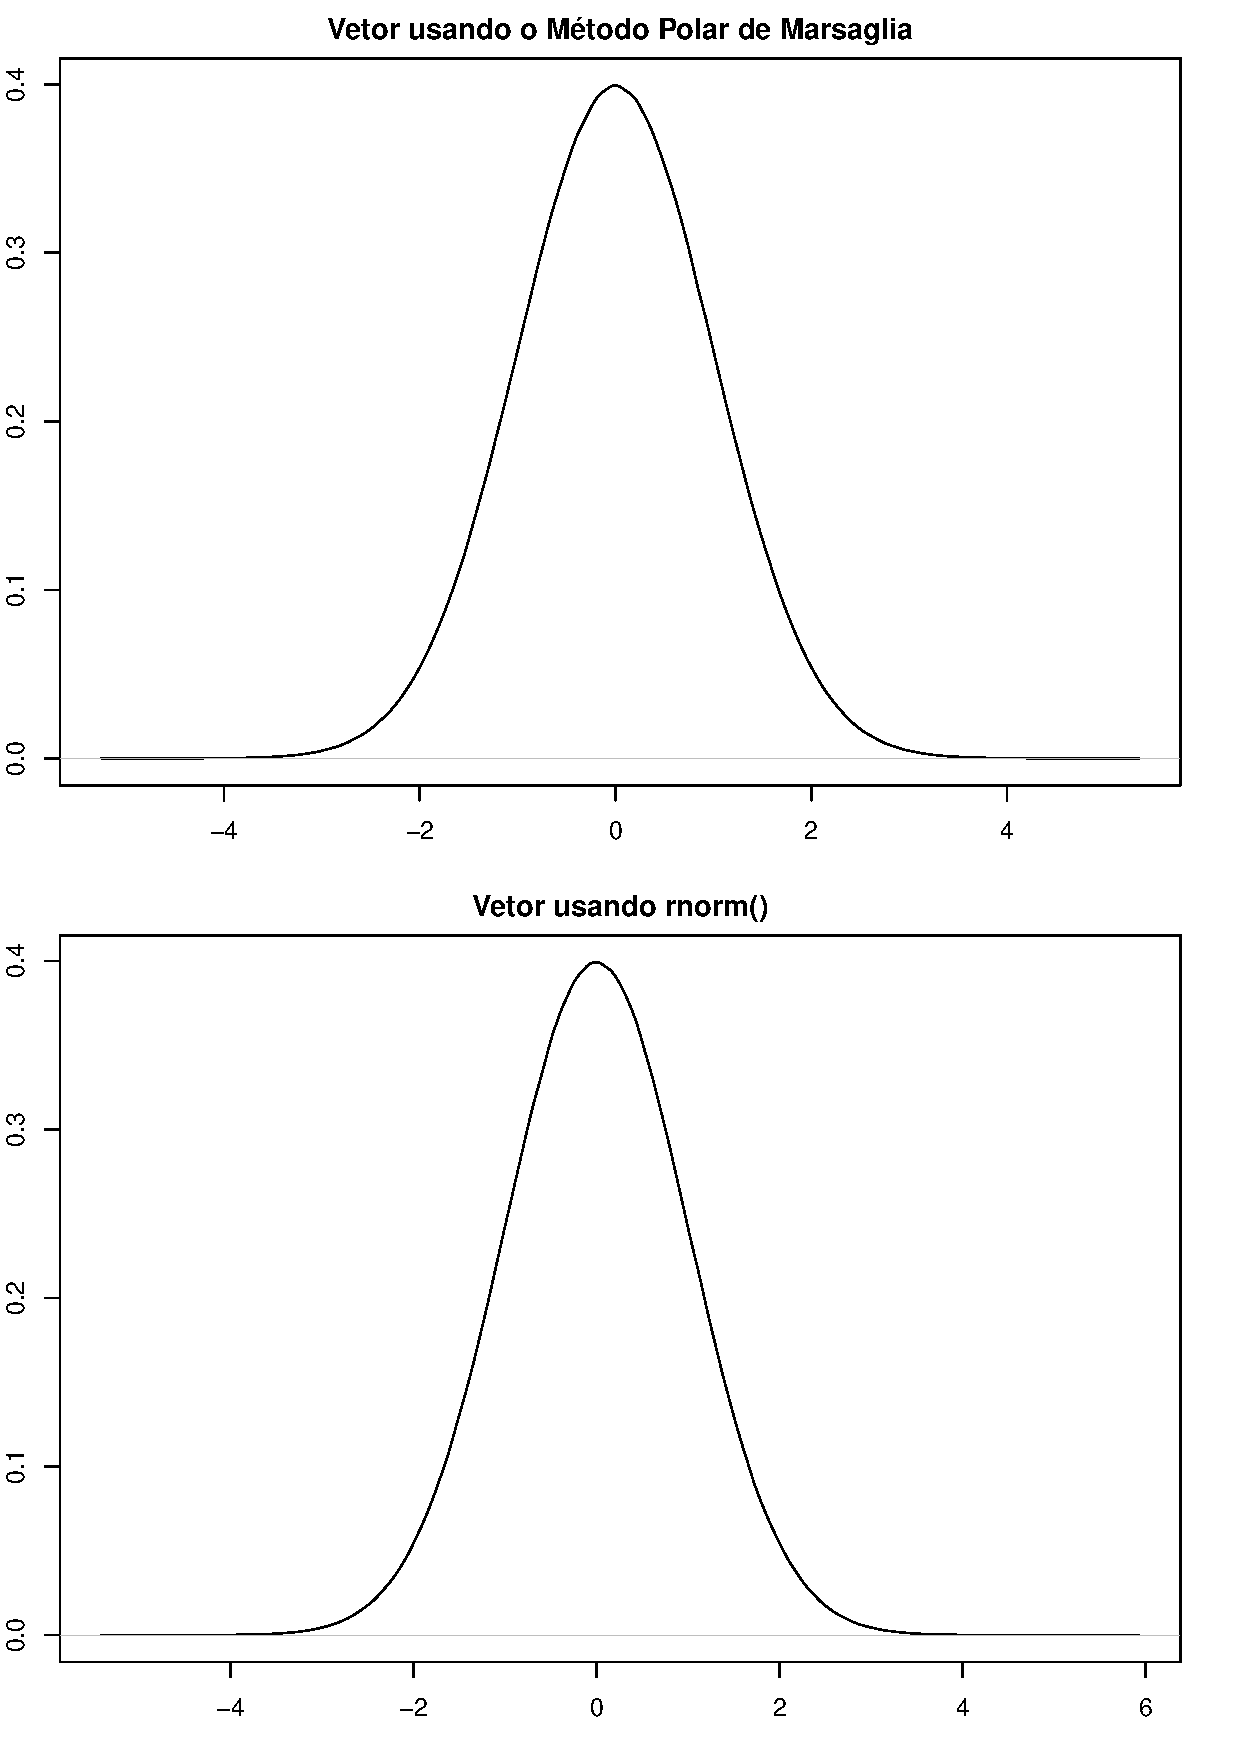
\includegraphics[scale=0.24]{rnorm_polar}
        \caption{Gráficos de Densidade \textit{Kernel} para o gerador que usa o Método Polar de Marsaglia e a para a função rnorm(), n = 10^7 em ambos}
        \label{fig:rnorm_polar}
    \end{figure}
    
    
\end{document}
